\documentclass[handout]{beamer}
\usepackage[utf8]{inputenc}
\usepackage{graphics}
\mode<presentation> {
\usetheme{unc}}
\setbeamertemplate{navigation symbols}{} % To remove the navigation symbols from the bottom of all slides uncomment this line

\usepackage{graphicx} % Allows including images
\usepackage{booktabs} % Allows the use of \toprule, \midrule and \bottomrule in tables


\usepackage{hyperref}
\hypersetup{linkcolor=blue,colorlinks=true}


% Remove symbols
\beamertemplatenavigationsymbolsempty


%\usetheme{default}

\usefonttheme{serif}

%----------------------------------------------------------------------------------------
%	TITLE PAGE
%----------------------------------------------------------------------------------------


\title[Grand Theories]{\LARGE{Grand Theories of International Relations}}
\author[POLI 150]{Steven Saroka}
\institute{POLI 150}
\date{23 January 2024}


\begin{document}

\begin{frame}
\titlepage % Print the title page as the first slide
\end{frame}


%\begin{frame}
%\frametitle{Overview} % Table of contents slide, comment this block out to remove it
%\tableofcontents % Throughout your presentation, if you choose to use \section{} and \subsection{} commands, these will automatically be printed on this slide as an overview of your presentation
%\end{frame}


%%% SLIDE TEMPLATES



% %% Core template for the slides

%----------------------------------------------------------------------------------------
%	PRESENTATION SLIDES
%----------------------------------------------------------------------------------------


%% Slide outline
\begin{frame} 
	\frametitle{\LARGE{Reminders}}
	\begin{itemize}
		\item Prompt 2 due Thursday night. 
		\\~\\ 
	\end{itemize}
\end{frame}

\begin{frame} 
	\frametitle{\LARGE{Today's Class}}
	\begin{itemize}
		\item Recap
		\\~\\ 
		\item Grand Theories and Their Use
		\\~\\ 
		\item Shift To Midrange Theories
		\\~\\ 
	\end{itemize}
\end{frame}

\begin{frame} 
	\frametitle{\LARGE{Central Questions}}
	\begin{center}
		\LARGE What are the Grand Theories of IR? 
		\LARGE How are these theories used in IR today? 
	\end{center}
\end{frame}

\begin{frame} 
	\frametitle{\LARGE{Key Terms}}
	\begin{itemize}
		\item Realism
		\item Liberalism
		\item Constructivism
		\item Midrange Theory 
	\end{itemize}
\end{frame}

\begin{frame} 
\frametitle{\LARGE{Foundational Concepts}}
    \begin{itemize}
        \item Politics: process by which scarce resources are allocated.
        \item Anarchy: no central authority above states in international politics.
        \item States: sovereign central authorities over a given territory with a monopoly on the use of force.
        \item Institutions: common sets of rules that order interactions.
        \item \textbf{International system/international order}: the way states fit together into a system, usually defined by \textbf{power}.
    \end{itemize}
\end{frame}

\begin{frame} 
\frametitle{\LARGE{Power}}
\begin{itemize}
    \item \textbf{Power}: the ability of one actor to get another actor to do something they would not ordinarily do. \pause
    \item Where does power come from? \pause
    \begin{itemize}
        \item Military resources \pause
        \item Economic size and diversity \pause
        \item Territory \pause
        \item Population \pause
        \item Fungibility (ability to turn the above into military strength) \pause
    \end{itemize}
    \item But where do those resources come from to begin with? \pause
    \item The state's ability to organize and tax within its territory, enabling it to mobilize these resources when needed.
    \begin{itemize}
    	\item ``War makes the state, and the state makes war" (Tilly 1979)
    \end{itemize}
\end{itemize}
\end{frame}

\begin{frame} 
\frametitle{\LARGE{Power}}
\begin{itemize}
    \item How do you exercise power? \pause
    \begin{itemize}
        \item Persuasion \pause
        \item Rewards \pause
        \item Threats \pause
        \item Non-violent punishments (sanctions, tariffs, etc.) \pause
        \item War \pause
    \end{itemize}
    \item How to tell when one state is more powerful? Hard to quantify, but political scientists have tried.
\end{itemize}
\end{frame}

\begin{frame} 
	\frametitle{\LARGE{Correlates of War Project: CINC Scores}}
	\begin{itemize}
		\item Correlates of War (COW) was started in 1963 by J. David Singer at the University of Michigan. \pause
		\item Goal: systematic accumulation of scientific knowledge about war. \pause
		\item Has since developed many useful quantitative conflict datasets (ex: Militarized Interstate Disputes; CINC Scores).
		\item CINC scores attempt to measure a state's military power.		
	\end{itemize}
\end{frame}

\begin{frame} 
	\frametitle{\LARGE{Correlates of War Project: CINC Scores}}
	\begin{itemize}
		\item CINC scores aggregate 6 indicators: \pause
		\begin{itemize}
			\item Military expenditure
			\item Military personnel
			\item Energy consumption
			\item Iron and steel production
			\item Urban population
			\item Total population \pause
		\end{itemize}	
		\item Higher CINC scores (in theory) indicate greater military power.	
	\end{itemize}
\end{frame}

\begin{frame} 
	\frametitle{\LARGE{2016 Global CINC Scores}}	
	\centering
	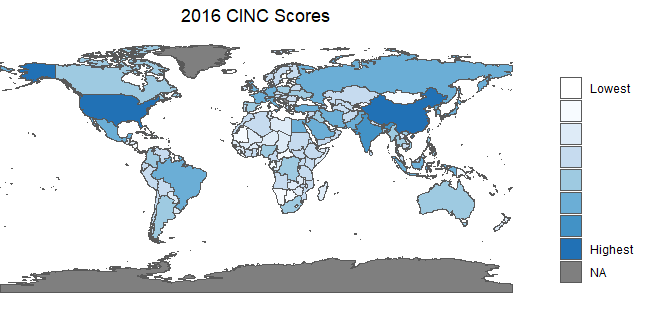
\includegraphics[width=\textwidth,height=0.9\textheight,keepaspectratio]{CINC2016.png}
\end{frame}


\begin{frame} 
	\frametitle{\LARGE{Explaining International Relations}}
	\begin{itemize}
	    \item All grand theories implicitly or explicitly draw on assumptions about human nature. \pause
	    \item The type of explanation a theory gives is heavily influenced by this starting assumption. \pause
	    \item \textbf{``Grand theories" attempted to explain everything about the international system, including how and why states wielded their power.} \pause
	    \item They have fallen from popularity in recent years, but they still have useful components. \pause
	    \item Most importantly, our ideas for how to explain world politics are built out of the elements of the grand theories, and informed by their failures.   
	\end{itemize}  
\end{frame}

\begin{frame} 
	\frametitle{\LARGE{Structure of This Lecture}}
	\begin{itemize}
	    \item What does the theory assume about human nature? \pause
	    \item What are its core components? \pause
	    \item Where did it come from? \pause
	    \item How was it useful? \pause
	    \item How has it failed? \pause
	    \item Running example: US decision to invade Iraq in 2003.
	\end{itemize}	  
\end{frame}


%% Part 2 - Realism

\begin{frame} 
\frametitle{\LARGE{Realism}}
``International politics, like all politics, is a struggle for power. Whatever the ultimate aims of international politics, power is always the immediate aim." \\
\hspace*{160pt} -Hans Morgenthau
\end{frame}


\begin{frame} 
\frametitle{\LARGE{Realism}}
\begin{itemize}
    \item Assumption about human nature: \pause other people can never be trusted. \pause 
    \item Thus, no actor can ever be sure they are safe. \pause
    \item The only way to ensure safety is through physical force (to have a strong military). \pause
    \item States, because of sovereignty, are the basic units that control militaries. \pause
    \item Therefore, states are the only actors that matter in world politics, because only they can guarantee this core need of safety via military power.
\end{itemize}
\end{frame}

\begin{frame} 
\frametitle{\LARGE{Realism}}
    \begin{itemize}
        \item States thus become the primary unit of analysis, and are viewed as the only actors that matter in our theories of politics. \pause
        \item States are assumed to be constantly focused on survival via increasing their security and power. \pause 
        \item To improve their security, they must improve military power. \pause 
        \item States interact in an anarchic world, with violence always possible. \pause
        \item Therefore, all world politics is bargaining under the shadow of conflict. 
    \end{itemize}
\end{frame}

\begin{frame} 
	\frametitle{\LARGE{Realism: Security Dilemmas}}
	\begin{itemize}
		\item States in a realist world often find themselves trapped in a \textbf{security dilemma}: defensive improvements to their military power due to this anarchy and uncertainty cause other states to fear those improvements will be used to attack them, leading those other states to improve their military capabilities. \pause
		\item Those improvements cause the first state to feel threatened, leading to arms races and potentially war.
	\end{itemize}
\end{frame}
       
        
        
\begin{frame} 
	\frametitle{\LARGE{Realism}}
	\begin{itemize}
		\item A main prediction of realism is \textbf{Balance of Power Theory}: Weaker states will improve their security by forming a balance of power, banding together with each other to ``balance" against stronger ones. \pause
		\item Another core assumption (borrowed from game theory and economics) is that states can be theorized as rational actors. \pause
		\item Structural factors of the international system mean that states in similar positions will behave similarly regardless of their domestic institutions.
	\end{itemize}
\end{frame}

\begin{frame} 
\frametitle{\LARGE{Realism}}
In sum: international relations is a Hobbesian state of nature in which every state is constantly measuring itself against others in terms of their ability to win wars. Rules, norms, institutions, even individuals don't matter - all that matters are states and security. \pause
\begin{itemize}
	\item Note how this sidelines international institutions and economic considerations.
\end{itemize}
\end{frame}

\begin{frame} 
\frametitle{\LARGE{History of Realist Thought}}
    \begin{itemize}
    	\item This pessimistic view of human relations is very old and very well-established.
        \item Thucydides (460---400 BCE): \pause ``Right, as the world goes, is only in question between equals in power, while the strong do what they can and the weak suffer what they must."
        \item Niccolò Machiavelli (1469---1527 CE): \pause ``Since love and fear can hardly exist together, if we must choose between them, it is far safer to be feared than loved.” 
        \item Carl von Clausewitz (1780---1831 CE): \pause ``War is nothing but a continuation of politics by other means." 
    \end{itemize}
\end{frame}

\begin{frame} 
\frametitle{\LARGE{Where does modern Realism come from?}}
    \centering
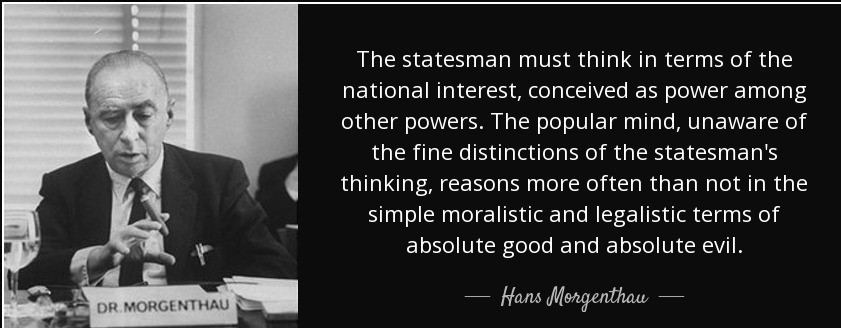
\includegraphics[width=\textwidth,height=0.8\textheight,keepaspectratio]{morgenthau.jpg}
Hans Morgenthau (1904---1980), especially \textit{Politics Among Nations} (1948)
\end{frame}

\begin{frame}{\LARGE Where does modern Realism come from?}
    \centering
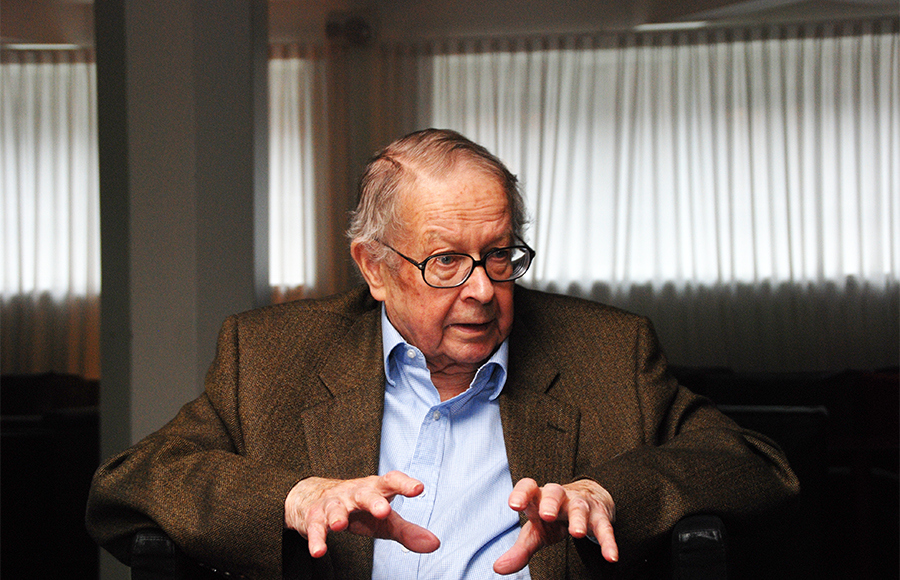
\includegraphics[width=\textwidth,height=0.8\textheight,keepaspectratio]{waltz.jpg}
Kenneth Waltz (1924---2013), especially \textit{Theory of International Politics} (1979)
\end{frame}

\begin{frame} 
\frametitle{\LARGE{How useful is Realism?}}
    \begin{itemize}
        \item Guides policymakers on avoiding war by assuming the worst (ideally). \pause
        \item Explains competition between great powers as due to insecurity. \pause
        \begin{itemize}
            \item Cold War \pause
            \item US---China? \pause
        \end{itemize}
        \item Iraq War: The centrality of military strength explains why the US was willing to resort to war against a weaker foe.
    \end{itemize}
\end{frame}

\begin{frame} 
\frametitle{\LARGE{How has Realism failed?}}
\begin{itemize}
    \item Internal flaw: Might assuming the worst make you less secure? Does this just trap states in a Prisoner's Dilemma of assuming the worst in any situation, missing opportunities for cooperation? \pause
    \item External flaws: \pause
    \begin{itemize}
        \item Completely failed to predict the fall of the USSR (major reputational blow). \pause
        \item Cannot describe why non-state actors (e.g. terrorists) are important. \pause
        \item Ignores role of international institutions as well as economic interests. \pause
        \item Indeterminate Balance of Power predictions.
    \end{itemize}
    \item Iraq War: \pause 
    \begin{itemize}
        \item Cannot explain why the U.S. was willing to use military might \textbf{at that moment}. 
    \end{itemize}
\end{itemize}
\end{frame}

% Liberalism

\begin{frame} 
\frametitle{\LARGE{Liberalism}}
``States do not typically cooperate out of altruism or empathy with the plight of others... They seek wealth and security for their own people, and search for power as a means to those ends." \\
\hspace*{160pt} -Robert Keohane
\end{frame}


\begin{frame} 
\frametitle{\LARGE{Liberalism}}
\begin{itemize}
    \item Assumption about human nature: \pause humans are basically trustworthy but also self-serving. \pause 
    \item Thus, humans care not only about their safety but also their welfare (generating wealth). \pause
    \item Thus, humans need both military security and economic growth. \pause
    \item Therefore, states are still the most important actors, but they are no longer the only actors worth examining.
    \item Scholars must also account for other actors that are relevant for the economy. \pause
    \item \textbf{International institutions are particularly important. Why?}
\end{itemize}
\end{frame}

\begin{frame} 
\frametitle{\LARGE{Liberalism}}
    \begin{itemize}
    	\item The primary goal of states is to amass wealth and grow their economy. \pause
    	\item International institutions can help with this, as they enable cooperation between states by setting rules and sharing information. \pause
        \item Economic interactions are generally about making both sides better off. \pause
        \item Thus, world politics is primarily about finding ways to enable cooperation. 
 \end{itemize}
\end{frame}

\begin{frame} 
	\frametitle{\LARGE{Liberalism}}
	\begin{itemize}
	   \item What about security? \pause
	   \item Wealth is required for any military, so even though states can care about security, they need to focus on gathering wealth to ensure their security.  \pause
	   \item States here are no longer solely focused on military power as the source of all strength. \pause
	   \item Thus, the international system is shaped not only by military power but also by economic power.  
	\end{itemize}
\end{frame}

\begin{frame} 
\frametitle{\LARGE{Liberalism}}
\begin{itemize}
	\item This focus on international economic activity means this theory accepts that non-state actors that have economic importance (international institutions, companies, domestic institutions) can influence international relations. \pause
	\item In sum: IR is about states as the primary - but not only - actors, trying to cooperate for economic gains. Conflict is ultimately the result of a failure to find a way to cooperate. 
\end{itemize}
\end{frame}

\begin{frame} 
\frametitle{\LARGE{Where does Liberalism come from?}}
    \centering
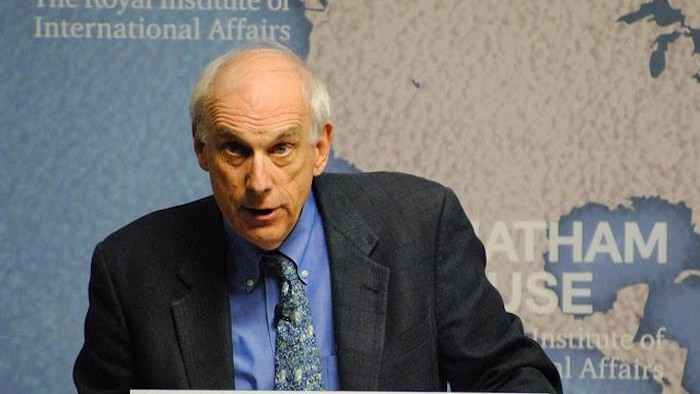
\includegraphics[width=\textwidth,height=0.8\textheight,keepaspectratio]{keohane.jpeg}
Robert Keohane (b. 1941), especially \textit{After Hegemony} (1984)
\end{frame}


\begin{frame} 
\frametitle{\LARGE{How useful is Liberalism?}}
    \begin{itemize}
        \item Incorporates other issues (esp. economics) that are clearly important to states besides security. \pause
        \item Helps to explain why international institutions exist at all. \pause
        \item Iraq War \pause 
        \begin{itemize}
            \item Explains why Bush and his administration tried to get UN approval before invading. 
        \end{itemize}
    \end{itemize}
\end{frame}

\begin{frame} 
\frametitle{\LARGE{How has Liberalism failed?}}
\begin{itemize}
    \item Overlooks the importance of zero-sum bargaining in politics. \pause
    \item Still cannot explain any real variations in outcomes in the international system. \pause
    \item Iraq War: \pause Doesn't explain why the US decided to invade despite failing to get approval from the UN (an international institution).
\end{itemize}
\end{frame}

% Constructivism

\begin{frame} 
\frametitle{\LARGE{Constructivism}}
``Anarchy is what states make of it." \\
\hspace*{160pt} -Alexander Wendt
\end{frame}


\begin{frame} 
\frametitle{\LARGE{Constructivism}}
\begin{itemize}
    \item Assumption about human nature: it is socially constructed. \pause 
    \item Human society, including IR, is all socially constructed. \textbf{This includes anarchy}. \pause
    \item The state is socially constructed from warfare, so it has a central place in world politics. \pause
    \item Thus, world politics is what states choose to make it, and there is no overriding logic for how states must behave. \pause 
    \item State behavior is shaped by the norms, beliefs, and identity of those within the state rather than just power considerations.
\end{itemize}
\end{frame}

\begin{frame} 
\frametitle{\LARGE{Constructivism}}
    \begin{itemize}
        \item Actors do what they think is appropriate (they follow rules). \pause 
        \item Ideas define the rules, so the rules can change over time as new ideas take root. \pause 
        \item Therefore, other actors besides states are extremely relevant for creating the ideas that drive the construction of the system. \pause
        \item International institutions and transnational actor networks (like non-governmental advocacy groups) can help create or change norms that constrain state behavior.
    \end{itemize}
\end{frame}

\begin{frame} 
	\frametitle{\LARGE{Constructivism}}
	\begin{itemize}
		\item Critiques the assumption of the other two theories that anarchy is inherently threatening.
		\item Argues that there is no inherent reason why lack of central authority is a problem. \pause
		\item Fears of violence and the need for security under anarchy are \textbf{assumptions} humans bring to the situation, not inherent aspects of the situation. 
	\end{itemize}
\end{frame}

\begin{frame} 
\frametitle{\LARGE{Constructivism}}
In sum: behavior in international relations is defined by rules, and rules are changed by ideas. Actors that  influence ideas - states, institutions, transnational actors - influence world politics. 

\end{frame}

\begin{frame} 
\frametitle{\LARGE{Where does Constructivism come from?}}
    \centering
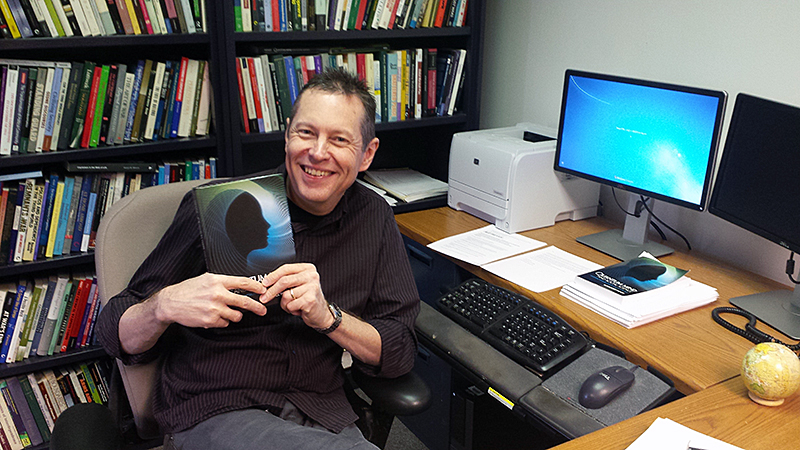
\includegraphics[width=\textwidth,height=0.8\textheight,keepaspectratio]{wendt.jpg}
Alexander Wendt (b. 1958), especially \textit{Social Theory of International Politics} (1999)
\end{frame}

\begin{frame} 
\frametitle{\LARGE{How useful is Constructivism?}}
    \begin{itemize}
        \item Oftentimes very descriptively accurate.  \pause
        \item Focus on ideas clarifies a focus on who has the power to set rules. \pause
        \item Adds stronger emphasis on the influence of non-state actors in spreading ideas. \pause
        \item Can explain how norms and practices change over time.
        \item Iraq War: suggests that the invasion occurs because the primary actors were driven by ideals. \pause
        \begin{itemize}
            \item US view of democracy as the best form of government. \pause
            \item US should rectify human rights abuses of Hussein's regime. \pause
            \item United States as the enforcer of world order.
          \end{itemize}
      \end{itemize}
\end{frame}

\begin{frame} 
\frametitle{\LARGE{How has Constructivism failed?}}
\begin{itemize}
    \item If human nature can be anything, this framework becomes so expansive as to explain very little of interest. \pause
    \item How often do these rules really change? \pause 
    \item Politics is especially difficult to study if you're concerned about actors' ideas and self-perceptions. 
    \item Iraq War: \pause 
    \begin{itemize}
        \item Again: why the invasion now? \pause
        \item How to explain all the materialistic rhetoric leading into the war? \pause
    \end{itemize}
\end{itemize}
\end{frame}

%%
\begin{frame} 
\frametitle{\LARGE{Where Are the Grand Theories Now?}}
\begin{itemize}
    \item So, where are these grand theories now? \pause
    \item While some still have adherents, most political scientists would not exclusively identify with any one of these camps. \pause
    \item Why? 
\end{itemize}
\end{frame}

\begin{frame} 
	\frametitle{\LARGE{The Fatal Flaw}}
	\begin{itemize}
		\item Each of these theories draws its explanatory power from factors which either don't change or are so expansive as to be useless analytically. Each struggles to explain changes in the international system (Snyder 2004). \pause
		\begin{itemize}
			\item Realism: If anarchy is constant, why does war happen in some cases but not others? If states are the only actors that matter, why do they spend so much time worrying about institutions? Why do specific balances of power form? \pause
			\item Liberalism: Why does cooperation fail sometimes? What does drive conflict in some cases but cooperation in others? \pause
			\item Constructivism: What drives human assumptions anyway?
		\end{itemize}
	\end{itemize}
\end{frame}

\begin{frame} 
	\frametitle{\LARGE{The Fatal Flaw}}
	\begin{itemize}
		\item Each of these grand theories struggled to explain why the Cold War ended, and why it ended the way it did. \pause
		\item \textbf{More fundamentally, their focus on the international system meant a lack of variance: the basic structure of the international order does not change much or frequently, but we observe lots of differing outcomes for states within that order.}
	\end{itemize}
\end{frame}
    
\begin{frame} 
	\frametitle{\LARGE{Shift to Midrange Theory}}
	\begin{itemize}
		\item General realization by political scientists that each of these theories had flaws, while failing to explain different outcomes at the state level. \pause
		\item Despite these flaws, they also recognized that these theories contained useful elements. \pause
		\item Thus, there was a shift away from ``grand" explanations of the entire international system to more ``midrange" explanations of specific phenomena. 
		\begin{itemize}
			\item Types of war, specific economic interactions, etc.
		\end{itemize}
	\end{itemize}
\end{frame}

\begin{frame} 
	\frametitle{\LARGE{Grand Theory Salvage}}
So, what did political scientists keep from these grand theories?
	\begin{itemize}
		\item From Realism: states as primary actors, importance of security, anarchy, strategic interactions. \pause
		\item From Liberalism: ability of international institutions to influence states, importance of economic activity, importance of nonstate actors like corporations. \pause
		\item From Constructivism: importance of the influence of starting assumptions.		
	\end{itemize}
\end{frame}

\begin{frame} 
	\frametitle{\LARGE{Midrange Theory Sampler}}
	What are some successful midrange theories?
	\begin{itemize}
		\item Bargaining model of war \pause
		\item Models of violence in civil wars \pause
		\item Theories of terrorism \pause
		\item Impact of domestic factors on both war and trade \pause
		\item Domestic and international political economy		
	\end{itemize}
\end{frame}

\end{document}